%% Seminar deck: Markovian and multi-curve friendly parametrisation of an
%% HJM model used in valuation adjustment of interest rate derivatives
%% (Bank i Kredyt, 2019). House style, academic register.
\documentclass[aspectratio=169,11pt]{beamer}
\usepackage{beamerthemeyc}
\renewcommand{\deckfootertitle}{Dec (2019) · Markovian multi-curve HJM for valuation adjustments · Bank i Kredyt}

\begin{document}

% 1 ---------------------------------------------------------------------------
\begin{frame}[plain]
  \vspace{2mm}
  {\ttfamily\scriptsize\color{ycmuted}SEMINAR DECK · YIELDCARTOGRAPHY.COM}\\[-0.3em]
  {\color{ycrule}\rule{\textwidth}{0.5pt}}
  \vspace{4mm}

  {\fontsize{18}{22}\selectfont\bfseries\color{ycink}Markovian and multi-curve friendly\\parametrisation of a HJM model used in\\valuation adjustment of interest rate derivatives.\par}
  \vspace{6mm}
  {\small\bfseries Marcin Dec\par}
  {\footnotesize\color{ycmuted}Kozminski University \& FAME|GRAPE, Warsaw\par}
  \vspace{3mm}
  {\ttfamily\scriptsize\color{ycaccent}Bank i Kredyt, 50(2), 2019 · bankikredyt.nbp.pl\par}
  \vfill
  \raisebox{-1mm}{
\includegraphics[height=6mm]{kozminski_logo.png}}\hspace{5mm}
  \raisebox{-1mm}{
\includegraphics[height=6mm]{grape_logo.png}}\hspace{5mm}
  \raisebox{-1mm}{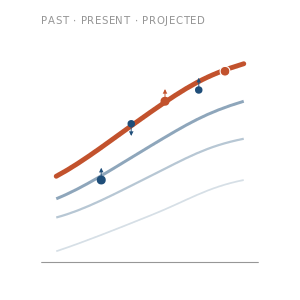
\includegraphics[height=6mm]{yc_logo.png}}
\end{frame}

% 2 ---------------------------------------------------------------------------
\begin{frame}{Motivation}
  \kicker{XVA needs a joint, simulable curve model}
  \begin{itemize}
    \item Valuation adjustments (CVA, DVA, FVA and related XVA terms) on
          interest-rate derivative portfolios require simulating the entire
          curve system, discounting and projection curves jointly, over long
          horizons and across collateralised and uncollateralised netting
          sets.
    \item The Heath--Jarrow--Morton framework prices consistently by
          construction, but a generic HJM volatility makes the forward-curve
          state non-Markovian, which is computationally prohibitive in an
          XVA engine.
    \item The paper constructs a parametrisation that is simultaneously
          Markovian and consistent with the post-crisis multi-curve setting.
  \end{itemize}
\end{frame}

% 3 ---------------------------------------------------------------------------
\begin{frame}{The HJM framework and the Markovian restriction}
  \kicker{Model class}
  \small Under the risk-neutral measure the instantaneous forward curve
  follows
  \[ df(t,T) \;=\; \alpha(t,T)\,dt + \sigma(t,T)\,dW_t,
     \qquad
     \alpha(t,T) \;=\; \sigma(t,T)\!\int_t^{T}\!\sigma(t,s)\,ds, \]
  the drift pinned down by no-arbitrage. A separable volatility structure,
  \( \sigma(t,T) = g(t)\,h(T) \), collapses the curve dynamics onto a
  finite-dimensional Markovian state.
  \begin{itemize}
    \item The paper works out a parametrisation in this class rich enough to
          fit the observed swap and OIS curve data while keeping the state
          vector small.
  \end{itemize}
\end{frame}

% 4 ---------------------------------------------------------------------------
\begin{frame}{Multi-curve consistency}
  \kicker{Discounting and projection after the crisis}
  \begin{itemize}
    \item Post-2008 markets separate the discounting curve (OIS,
          collateral-rate based) from tenor-specific projection curves, with
          non-negligible basis between them.
    \item The parametrisation is built to be multi-curve friendly: the
          discount and projection layers are modelled consistently, so
          collateralised and uncollateralised trades are valued within one
          engine.
    \item The result is a state-space small enough for the nested
          simulations of XVA while preserving the fit to the swap-curve and
          OIS-curve data.
  \end{itemize}
\end{frame}

% 5 ---------------------------------------------------------------------------
\begin{frame}{Implications}
  \kicker{For XVA practice}
  \begin{itemize}
    \item Dimensionality reduction is obtained by parametric structure
          instead of ad-hoc factor truncation, so the no-arbitrage
          consistency of HJM is retained inside the XVA engine.
    \item The framework covers collateralised and uncollateralised
          interest-rate derivatives in one model, which is precisely the
          portfolio mix on which valuation adjustments are computed.
    \item The construction predates and complements the later LLM
          yield-curve programme: the same discipline of explicit
          parametrisation over convention.
  \end{itemize}
\end{frame}

% 6 ---------------------------------------------------------------------------
\begin{frame}[plain]
  \vspace{12mm}
  {\fontsize{27}{31}\selectfont\bfseries\color{ycink}Thank you.\par}
  \vspace{6mm}
  {\normalsize\color{ycink}Marcin Dec\par}
  {\small\color{ycmuted}Kozminski University \& FAME|GRAPE, Warsaw\\
   mdec@kozminski.edu.pl · ORCID 0000-0002-6220-8267\par}
  \vspace{5mm}
  {\ttfamily\footnotesize\color{ycaccent}%
   Dec, M. (2019). Markovian and Multi-Curve Friendly Parametrisation\\
   of a HJM Model Used in Valuation Adjustment of Interest Rate\\
   Derivatives. Bank i Kredyt, 50(2) · bankikredyt.nbp.pl\par}
  \vfill
  \raisebox{-1mm}{
\includegraphics[height=6mm]{kozminski_logo.png}}\hspace{5mm}
  \raisebox{-1mm}{
\includegraphics[height=6mm]{grape_logo.png}}\hspace{5mm}
  \raisebox{-1mm}{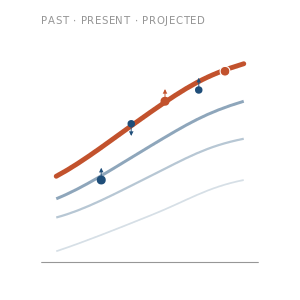
\includegraphics[height=6mm]{yc_logo.png}}
  \hfill{\ttfamily\scriptsize\color{ycmuted}yieldcartography.com/slides/hjm/}
\end{frame}

\end{document}
